\documentclass{article}%
\usepackage[T1]{fontenc}%
\usepackage[utf8]{inputenc}%
\usepackage{lmodern}%
\usepackage{textcomp}%
\usepackage{lastpage}%
\usepackage[head=40pt,margin=0.5in,bottom=0.6in]{geometry}%
\usepackage{graphicx}%
%
\title{\textbf{Maestros declararon en emergencia al sector educativo}}%
\author{EFE}%
\date{01/10/2018}%
%
\begin{document}%
\normalsize%
\maketitle%
\textbf{URL: }%
http://www.el{-}nacional.com/noticias/protestas/maestros{-}declararon{-}emergencia{-}sector{-}educativo\_253866\newline%
%
\textbf{Periodico: }%
EN, %
ID: %
253866, %
Seccion: %
Protestas\newline%
%
\textbf{Palabras Claves: }%
Educación, Nicolás Maduro, Sociedad\newline%
%
\textbf{Derecho: }%
2.2, %
Otros Derechos: %
, %
Sub Derechos: %
2.2.1.1\newline%
%
\textbf{EP: }%
NO\newline%
\newline%
%
\textbf{\textit{Los profesionales de la educación señalaron que las infraestructuras escolares no fueron arregladas durante el período vacacional~}}%
\newline%
\newline%
%
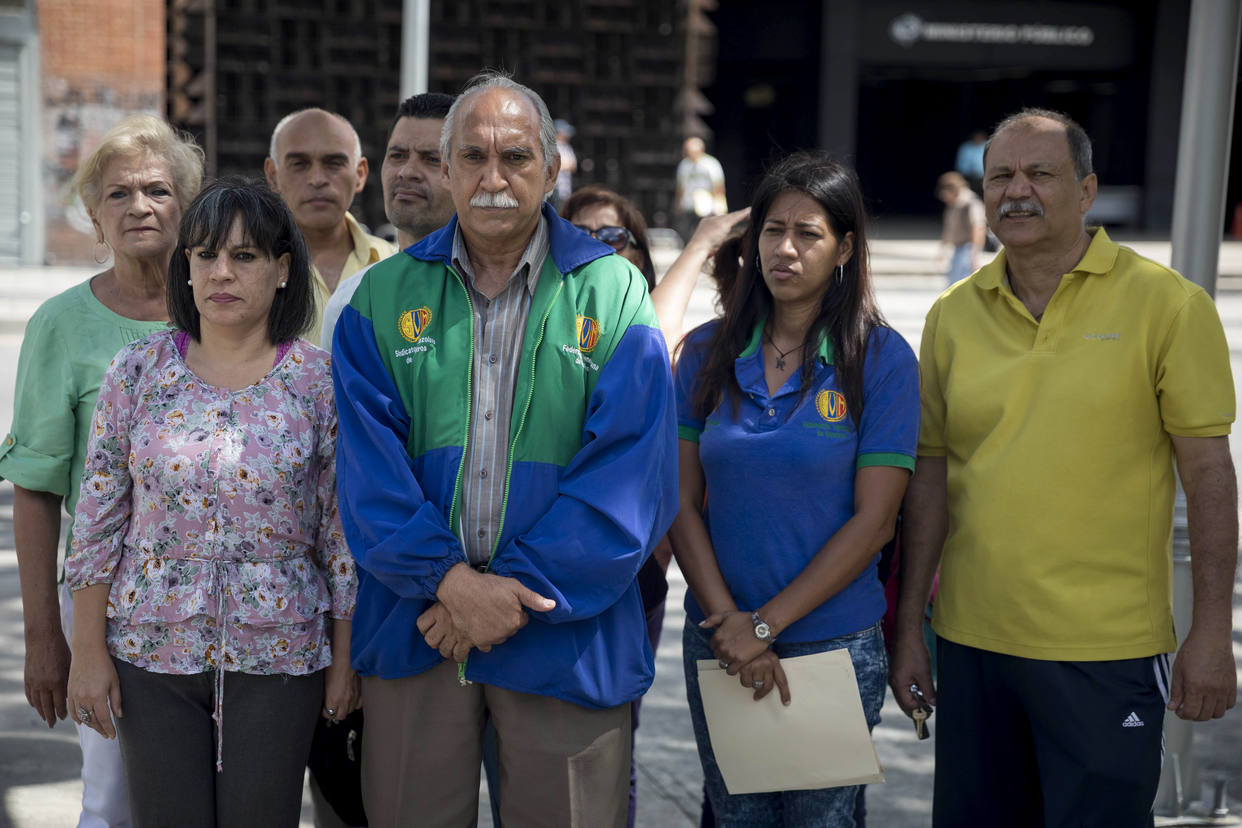
\includegraphics[width=300px]{170.jpg}%
\newline%
%
Maestros declararon este lunes la emergencia del sector educativo primario, que comenzó actividades hace una semana, y anunciaron que tomarán “acciones sindicales” si los pedidos de aumento salarial y mejores condiciones laborales no son atendidos.%
\newline%
%
Édgar Machado, presidente del sindicato de maestros de Caracas, dijo que el sector está en emergencia educativa~por la infraestructura de las instituciones que no fueron arregladas durante las vacaciones y por el salario de los maestros.%
\newline%
%
"Los educadores de Caracas estamos cansados, estamos en una emergencia educativa", aseguró Machado en una protesta.%
\newline%
%
El dirigente sindical señaló que el Estado incumplió al menos 8 términos del contrato colectivo que se firmó con los educadores.%
\newline%
%
"El presidente Nicolás Maduro se cansó de decir que era el mejor contrato para maestros a nivel mundial, entonces si es el mejor contrato, que se cumpla", añadió Machado.%
\newline%
%
"El sueldo no nos alcanza ni para poder sobrevivir. La calidad de vida de los educadores ha decaído totalmente, no tenemos ni para comprar el zapato más económico", señaló Machado.%
\newline%
%
\end{document}